% !TEX TS-program = xelatex
% !TEX encoding = UTF-8 Unicode
% !Mode:: "TeX:UTF-8"
\documentclass[14pt]{resume}
\usepackage{graphicx}
\usepackage{tabu}
\usepackage{multirow}
\usepackage{multicol}
\usepackage{progressbar}
\usepackage{zh_CN-Adobefonts_external}
\usepackage{linespacing_fix}
\usepackage{cite}

\begin{document}
\pagenumbering{gobble}

\begin{multicols}{4}
    \Large{
        \begin{tabu}{ r }
            \multirow{5}{1in}{
                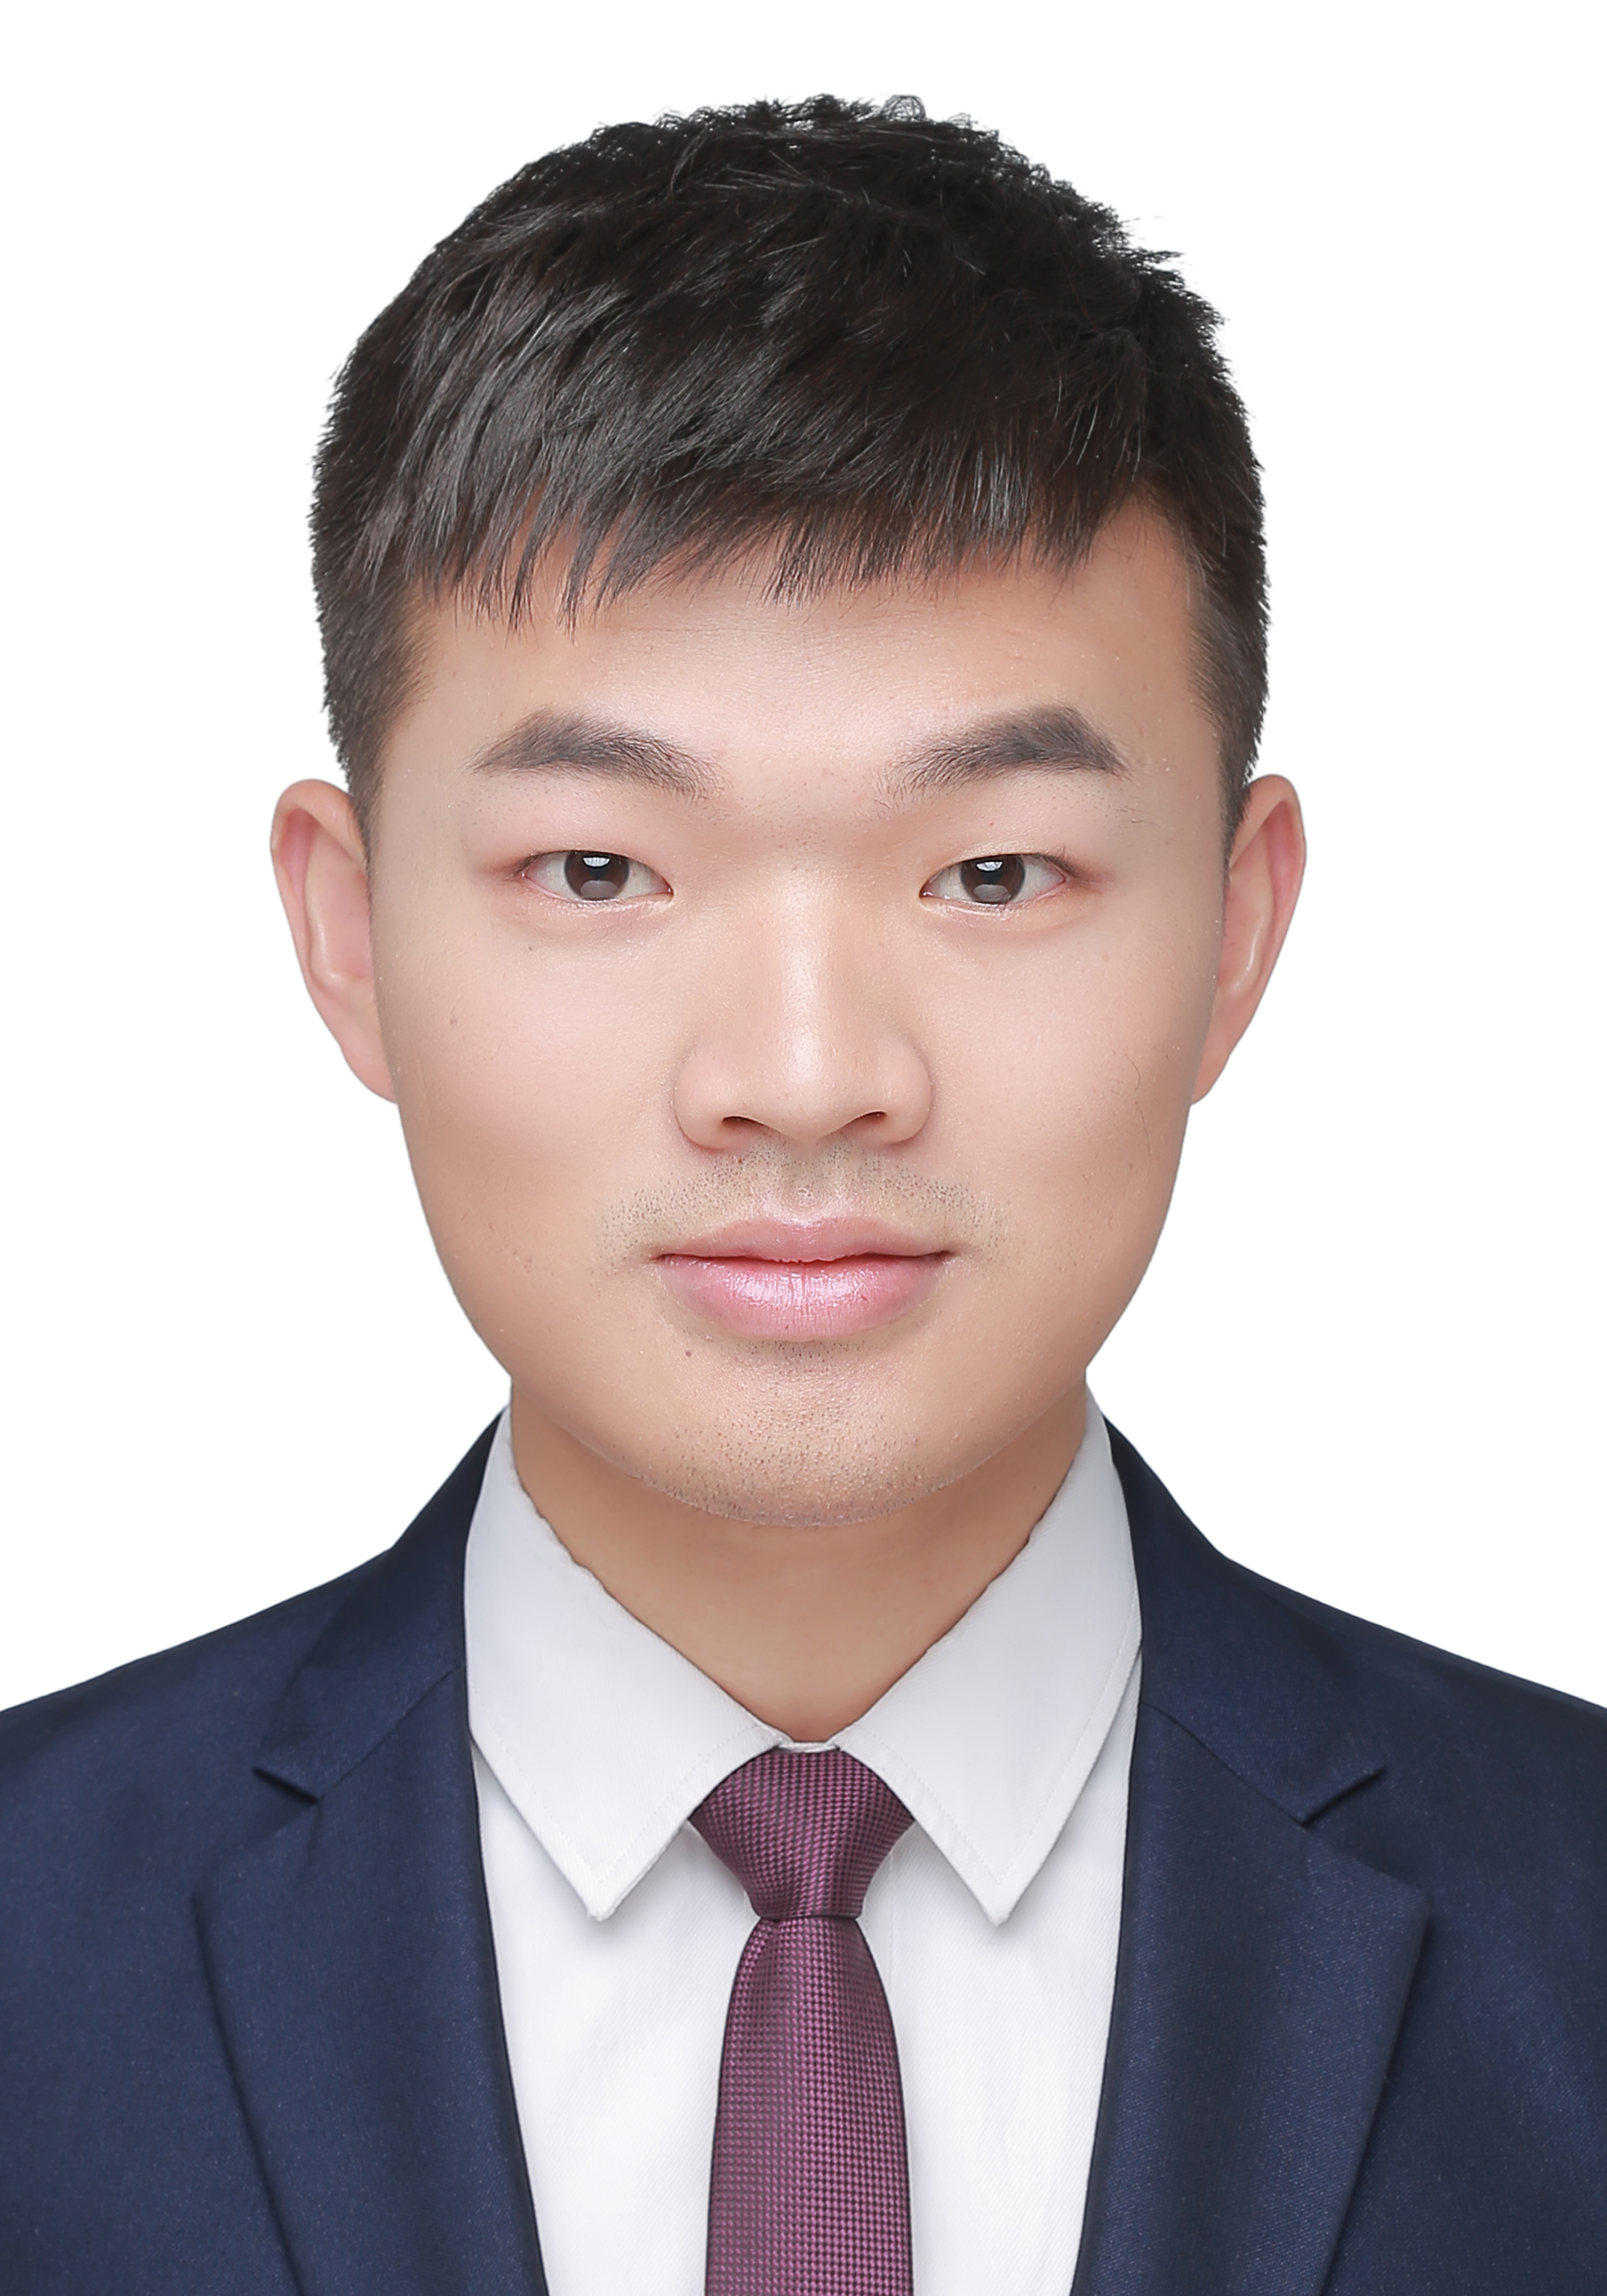
\includegraphics[width=0.88in]{avatar}
            }
        \end{tabu}
    }
    \columnbreak
    \Large{
        \begin{tabu}{ l l }
            & \faBirthdayCake{1995.09.12} \\
            & \phone{(+86)17600535912} \\
            & \email{izhouwl@163.com} \\
            & \homepage[www.zhouweilin.cn]{https://zhouweilin.cn} \\
            & \github[github.com/Si3ver]{https://github.com/Si3ver} 
        \end{tabu}
    }
    \columnbreak
    \Large{
        \begin{tabu}{ r }
            \multirow{5}{3.5in}{
                \name{周伟林}
                \basicInfo{
                    \faSmileO{意向职位:web前端研发}
                }
            }
        \end{tabu}
    }
\end{multicols}

% 教育背景
\section{\faGraduationCap\  教育背景}
\datedsubsection{\textbf{北京邮电大学(硕士)\quad\quad\quad}{ 网络技术研究院 \quad\quad\quad }{ 计算机科学与技术 }}{2016.09 - 2019.06}
\datedsubsection{\textbf{北京工业大学(本科)\quad\quad\quad}{ 计算机学院     \quad\quad\quad\quad\quad}{ 信息安全 }}{2012.09 - 2016.06}

% 技能树
\section{\faCogs\ 技能树}

\begin{itemize}
    \item[\faTree] 熟悉HTML、CSS、JavaScript,会使用ECharts、Bootstrap、jQuery,Canvas、AntD等
    \item[\faTree] 熟悉Vue.js,了解React.js
    \item[\faTree] 熟悉前后端分离、前端工程化的开发方式,了解前端性能优化
    \item[\faTree] 熟悉python语言,了解数据可视化,会使用Matplotlib、Markdown、LaTex\footnote{本简历使用LaTex书写并编译}
    \item[\faTree] 网络基础良好,熟悉HTTP(S)、TCP/IP,了解运营商技术,有网络运维相关经验
    \item[\faTree] 无障碍阅读英文文档(CET-6),熟练使用Google、Stack Overflow检索
\end{itemize}

% 实习经历
\section{\faBriefcase\ 实习经历}
\datedsubsection{\textbf{滴滴出行\quad\quad\quad\quad\quad} \textbf{质量技术部\quad\quad\quad\quad}{ WEB前端研发}}{2018.05 - 2018.09}
\begin{itemize}
    \item[\faFlagO] 参与月光宝盒(订单流量重放平台)和Omega(移动数据管理平台)两个项目的前端部分开发\footnote{图标说明,小旗图标表示项目/工作描述,代码图标表示个人工作/职责,对勾图标表示项目/工作成果}
    \item[\faFlagO] 使用原生JS、模板引擎Simplite、Less、jQuery、BootStrap、ECharts等工具开发
    \item[\faCode] 我负责客服反馈处理页、启动崩溃分析列表页与详细页等页面开发
    \item[\faCode] 为页面增加列表筛选过滤、语言切换等功能
    \item[\faCode] 使用ECharts库,为页面添加折线图、柱状图、饼图
    \item[\faCode] 代码重构。tree-shaking,拆分冗长代码,增加报错信息,与后端合作合并部分过于细分的API
    \item[\faCheck] 页面上线到正式系统中,供公司内部使用;提高代码可维护性和可重用性
\end{itemize}

\datedsubsection{\textbf{西门子中国\quad\quad\quad\quad} \textbf{新闻传播部\quad\quad\quad\quad}{网站技术支持}}{2017.10 - 2018.03}
\begin{itemize}
    \item[\faFlagO] 参与CMS内容迁移(官网新闻发布平台,从SharePoint迁移到AEM)项目
    \item[\faFlagO] 原系统由ASP页面构成,新系统基于H5,迁移需要重写部分布局和前端组件
    \item[\faCode] 开发Slider组件,用以展示最新图片及公司公开刊物,并通过iframe嵌入到原页面内
    \item[\faCode] 获取网站埋点数据的统计结果,整理每月PV/UV报表数据
    \item[\faCheck] 使用英文书面沟通,与老外口语交流;接触到大型新闻发布系统的运维
\end{itemize}

\datedsubsection{\textbf{北京江南天安科技\quad} \textbf{软件研发部\quad\quad\quad\quad}{Windows程序开发}}{2015.07 - 2015.09}
\begin{itemize}
    \item[\faFlagO] 密码机是公司的重要产品,本人参与一款UKey软件的windows开发部分
    \item[\faCode] 参与云密码机的专用UKey初始化工具、双因子认证软件的PC客户端开发
    \item[\faCheck] 熟悉了windows程序设计,熟练了VS的调试工具;加深了对安全通信和密码学的理解
\end{itemize}

% 项目经历
\section{\faUsers\ 项目经历}

\datedsubsection{\textbf{网络优化模型和算法\quad\quad\quad\quad\quad\quad}{设计、实现与仿真}}{2018.07 - 2017.09}
\begin{onehalfspacing}
\begin{itemize}
    \item[\faFlagO] 本项目属于实验室科研项目,研究内容为网络功能虚拟化场景下的VNF放置算法
    \item[\faFlagO] 经过调研发现,实际流量经常发生激增现象,导致丢包,会严重影响QoS
    \item[\faFlagO] 在VNFaaS部署到数据中心拓扑的前,可事先根据流量涨幅和突发概率的特征,据此建模来优化部署网络应用
    \item[\faCode] 在导师和实验室博士后师兄的指导下,完成了方案设计、代码实现和论文撰写
    \item[\faCheck] 用python实现了VNF放置算法的仿真环境NFVsimu,并在github开源
    \item[\faCheck] 抽象出了可扩展性的最优化模型,并证明其等价于二分匹配的子问题
    \item[\faCheck] 设计并实现了sVNFP和sVNFP-adv两个启发式算法,使丢包率降低了15\%-40\%
\end{itemize}
\end{onehalfspacing}

\datedsubsection{\textbf{SPA应用:去旅行\quad\quad\quad\quad\quad\quad\quad\quad}{Webapp开发}}{2018.04 - 2018.06}
\begin{onehalfspacing}
\begin{itemize}
    \item[\faFlagO] 基于Vue技术栈,仿造去哪儿网开发了一个名叫“去旅行”的移动端webapp
    \item[\faFlagO] 首页包含Header组件、轮播图、图标栏、热销推荐栏、周末游组件,还包括城市选择页、详情页等
    \item[\faFlagO] 前后端分离,Mock json数据,使用了axios、vuex、vue-router、better-scroll、H5 localStorage等工具
    \item[\faCode] 在线获取素材、阅读Vue文档,自行编码开发并开源到github
    \item[\faCheck] 熟悉了Vue框架,丰富了自己移动端的开发经验
\end{itemize}
\end{onehalfspacing}

\datedsubsection{\textbf{别踩白块儿\quad\quad\quad\quad\quad\quad\quad\quad}{移动端H5游戏开发}}{2018.01 - 2018.02}
\begin{onehalfspacing}
\begin{itemize}
    \item[\faFlagO] 基于canvas,游戏数据为四行四列的矩阵,以MVC设计模式组织代码
    \item[\faFlagO] 采用响应式布局,支持移动端touch事件
    \item[\faCode] 实现了别踩白块儿移动端小游戏,手机浏览器输入URL即玩
    \item[\faCheck] 丰富了自己移动端游戏开发经验
\end{itemize}
\end{onehalfspacing}

% 校园经历
\section{\faUniversity\ 校园经历}

\datedsubsection{\textbf{组织校园读书文化节活动\quad\quad\quad\quad\quad\quad\quad}{校学生会学拓部部员}}{2013.03 - 2013.05}
\begin{onehalfspacing}
\begin{itemize}
    \item[\faFlagO] 制作移动端web pages宣传页,用以收集同学书籍喜好和闲置书籍,组织书籍交换活动
    \item[\faFlagO] 组织趣味问答环节,答对问题数量越多,奖品越丰厚
    \item[\faFlagO] 组织队员制作路展物件,用印制板制作书形道具
    \item[\faFlagO] 路展过程中,收集同学们的书籍推荐词,用书签的方式贴到道具上
\end{itemize}
\end{onehalfspacing}

% 个人荣誉
\section{\faHeartO\ 个人荣誉}

\trophy [Weilin Zhou, Yuan Yang, Mingwei Xu, and Hao Chen, Accommodating dynamic traffic immediately: a VNF placement approach\footnote{ICC 2019评审中,CCF C类会议}]{https://github.com/Si3ver/SVNF}

\trophy [周伟林, 杨芫, 徐明伟. 网络功能虚拟化技术研究综述. 计算机研究与发展, 2018, 55(4): 675-688\footnote{国内计算机领域三大核心期刊之一,EI检索}]{http://crad.ict.ac.cn/CN/abstract/abstract3662.shtml}

\trophy [2015全国大学生网络技术大赛(思科网院杯),全国二等奖,排名第12]{http://www.catc.edu.cn/2015cup/news/19rr5gvqfnqk2.xhtml}

\trophy [北京邮电大学研究生一等学业奖学金、网研院优秀研究生]{xxx}

\trophy [北京工业大学学习优秀奖、科技创新奖、优秀毕业生、基础课奖学金,物理知识竞赛优等奖]{xxx}

% 特长爱好 + 自我评价
\section{\faInfo\ 关于我}

\faTerminal 热爱技术,关注新鲜事物

\faBook 爱好阅读和电影,偏爱历史类作品,也阅读了部分文学名著,对经济学、心理学也有部分了解

\faBicycle 喜欢户外运动,曾徒步登泰山、恒山,慕田峪、箭扣、墙子路。与小伙伴一天内骑车160公里从京城到京郊游玩

\faHeartbeat 坚持游泳,偶尔也打打羽毛球、乒乓球

\end{document}
